\label{chap:system_architecture}

\section{Introduction}
To bridge the operational intelligence gap between raw aerial remote sensing and accountable emergency disaster decision-making, the \textbf{FloodSense} framework is conceptualized as an integrated, three-tier multimodal architecture. This chapter establishes the rigorous mathematical foundations governing multi-class aerial semantic segmentation, quantitative infrastructure damage extraction, and semantic vector retrieval. Subsequently, it presents the architectural blueprint, data flow dynamics, and component interactions of the complete end-to-end system.

\section{Mathematical Problem Formulation}

\subsection{Multi-Class Semantic Segmentation Formulation}
Let an ultra-high-resolution aerial drone orthophoto be represented as a continuous three-channel tensor:
\begin{equation}
    \mathcal{I} \in \mathbb{R}^{3 \times H \times W}
\end{equation}
where $H$ and $W$ denote the image height and width in pixels (typically $H = 3000, W = 4000$ for native 12-megapixel UAV sensors), and each pixel coordinate $(x, y)$ contains standardized RGB radiance values normalized by the ImageNet mean $\boldsymbol{\mu} = [0.485, 0.456, 0.406]^T$ and standard deviation $\boldsymbol{\sigma} = [0.229, 0.224, 0.225]^T$.

Let $\mathcal{C} = \{0, 1, 2, \dots, C-1\}$ denote the discrete set of $C = 10$ mutually exclusive semantic land-cover and disaster impact classes defined by the FloodNet benchmark:
\begin{equation}
    \mathcal{C} = \left\{
    \begin{array}{ll}
        0: \text{Background}, & 1: \text{Building-Flooded}, \\
        2: \text{Building-Non-Flooded}, & 3: \text{Road-Flooded}, \\
        4: \text{Road-Non-Flooded}, & 5: \text{Water}, \\
        6: \text{Tree}, & 7: \text{Vehicle}, \\
        8: \text{Pool}, & 9: \text{Grass}
    \end{array}
    \right\}
\end{equation}

The ground truth segmentation mask is defined as a discrete spatial lattice:
\begin{equation}
    \mathcal{Y} \in \mathcal{C}^{H \times W}, \quad \text{where } y_{i} \in \mathcal{C} \text{ for each pixel } i \in \{1, \dots, N\} \text{ and } N = H \times W.
\end{equation}

The objective of the segmentation stage is to parameterize a deep neural mapping $f_{\boldsymbol{\theta}}: \mathcal{I} \rightarrow [0, 1]^{C \times H \times W}$, parameterized by weights $\boldsymbol{\theta}$, that maps the input image tensor $\mathcal{I}$ into a class probability distribution tensor $\mathbf{P}$:
\begin{equation}
    \mathbf{P} = f_{\boldsymbol{\theta}}(\mathcal{I}), \quad \text{such that } \sum_{c=0}^{C-1} p_{i, c} = 1 \quad \forall i \in \{1, \dots, N\}
\end{equation}
where $p_{i, c}$ denotes the predicted probability that pixel $i$ belongs to semantic class $c$. The final discrete prediction mask $\hat{\mathcal{Y}} = \{\hat{y}_i\}_{i=1}^N$ is obtained via maximum a posteriori (MAP) assignment:
\begin{equation}
    \hat{y}_i = \arg\max_{c \in \mathcal{C}} p_{i, c}
\end{equation}

The overall optimization goal is to discover optimal network parameters $\boldsymbol{\theta}^*$ that maximize the multi-class Mean Intersection over Union (mIoU / Jaccard Index):
\begin{equation}
    \boldsymbol{\theta}^* = \arg\max_{\boldsymbol{\theta}} \frac{1}{|\mathcal{C}_{valid}|} \sum_{c \in \mathcal{C}_{valid}} \frac{\sum_{i=1}^N \mathbb{I}(y_i = c \land \hat{y}_i = c)}{\sum_{i=1}^N \mathbb{I}(y_i = c \lor \hat{y}_i = c)}
\end{equation}
where $\mathbb{I}(\cdot)$ is the indicator function, and $\mathcal{C}_{valid}$ represents the subset of classes present in the ground truth or prediction.

\subsection{Quantitative Damage Metric Extraction Formulation}
Raw discrete prediction masks $\hat{\mathcal{Y}}$ are transformed into physically grounded damage metrics through spatial aggregation and morphological connected component analysis. Given the camera's Ground Sample Distance (GSD, measured in meters per pixel), the physical surface area $A_c$ (in square meters) occupied by semantic class $c$ is:
\begin{equation}
    A_c = \left( \sum_{i=1}^N \mathbb{I}(\hat{y}_i = c) \right) \cdot \text{GSD}^2
\end{equation}

For discrete civil infrastructure elements, let $\mathcal{B} = \{b_1, b_2, \dots, b_K\}$ denote the set of segmented building footprint polygons extracted via 8-connectivity component labeling over classes $\{1, 2\}$. Each building polygon $b_k$ is classified as flooded if its interior boundary contains water or is assigned to class $1$:
\begin{equation}
    N_{bld, flooded} = \sum_{k=1}^K \mathbb{I}\left( \text{Class}(b_k) = 1 \right), \quad N_{bld, total} = K
\end{equation}
The structural building inundation ratio $R_{building}$ is defined as:
\begin{equation}
    R_{building} = \frac{N_{bld, flooded}}{\max(1, N_{bld, total})} \in [0, 1]
\end{equation}

Similarly, the transportation network impassability ratio $R_{road}$ represents the proportion of road surfaces submerged under water:
\begin{equation}
    R_{road} = \frac{A_{\text{Road-Flooded}}}{A_{\text{Road-Flooded}} + A_{\text{Road-Non-Flooded}} + \epsilon} \in [0, 1]
\end{equation}
where $\epsilon = 10^{-7}$ prevents division by zero in regions devoid of road networks.

The vehicle entrapment metric $N_{veh}$ represents the count of detected vehicles (class 7) that are either fully submerged or directly adjacent (within a morphological dilation kernel of radius $r=15$ pixels) to flooded roads or water bodies.

\subsection{Composite Disaster Severity Index}
To provide incident commanders with an immediate, normalized priority metric, FloodSense computes a deterministic, multi-criteria \textbf{Disaster Severity Score} $S_{severity} \in [0, 100]$:
\begin{equation}
    S_{severity} = \min\left(100, \; 40 \cdot R_{building} + 35 \cdot R_{road} + 15 \cdot \min(1.0, \frac{N_{veh}}{5}) + 10 \cdot \frac{A_{water}}{A_{total}}\right)
\end{equation}
The continuous score $S_{severity}$ is categorized into standard FEMA/NDMA operational severity tiers:
\begin{equation}
\label{eq:severity_tier}
\resizebox{0.95\textwidth}{!}{$
\displaystyle
\text{Severity Tier} = \left\{
\begin{array}{lll}
    \textbf{Catastrophic (Level 4)} & \text{if } S_{severity} \ge 75 & \rightarrow \text{Immediate air/boat rescue deployment} \\
    \textbf{High (Level 3)} & \text{if } 50 \le S_{severity} < 75 & \rightarrow \text{Evacuation of ground floors \& medical aid} \\
    \textbf{Moderate (Level 2)} & \text{if } 25 \le S_{severity} < 50 & \rightarrow \text{Road clearance \& pump drainage} \\
    \textbf{Low (Level 1)} & \text{if } S_{severity} < 25 & \rightarrow \text{Precautionary monitoring \& vigilance}
\end{array}
\right.
$}
\end{equation}

\subsection{Mathematical Formulation of Semantic Vector Retrieval (RAG)}
Let the statutory disaster knowledge repository be partitioned into $M$ discrete, semantically coherent text chunks $\mathcal{D} = \{d_1, d_2, \dots, d_M\}$. Using a dense pre-trained bi-encoder embedding model $\Phi: \text{Text} \rightarrow \mathbb{R}^D$ (Sentence-BERT / \texttt{all-MiniLM-L6-v2}, $D = 384$), each document chunk is mapped to a normalized dense vector:
\begin{equation}
    \mathbf{e}_{d_m} = \frac{\Phi(d_m)}{\|\Phi(d_m)\|_2} \in \mathbb{R}^D, \quad \forall m \in \{1, \dots, M\}
\end{equation}
These vectors are indexed in a high-dimensional ChromaDB vector store.

When damage extraction produces physical metrics $\{R_{building}, R_{road}, N_{veh}, S_{severity}\}$, the query formulation engine generates an operational natural language query $q$. The query is embedded via the same encoder:
\begin{equation}
    \mathbf{e}_q = \frac{\Phi(q)}{\|\Phi(q)\|_2} \in \mathbb{R}^D
\end{equation}
The retriever performs Maximum Inner Product Search (MIPS) using cosine similarity:
\begin{equation}
    \text{sim}(q, d_m) = \mathbf{e}_q^T \mathbf{e}_{d_m} = \cos(\theta_{\mathbf{e}_q, \mathbf{e}_{d_m}})
\end{equation}
The top-$k$ relevant statutory protocol chunks $\mathcal{D}_{top-k} = \{d_{(1)}, \dots, d_{(k)}\}$ are retrieved to condition the final LLM synthesis prompt.

\section{End-to-End System Architecture Blueprint}
The FloodSense architecture is partitioned into three decoupled, high-performance tiers, as depicted in the architectural schematic in Figure~\ref{fig:system_architecture}:

\begin{figure}[htbp]
	\centering
	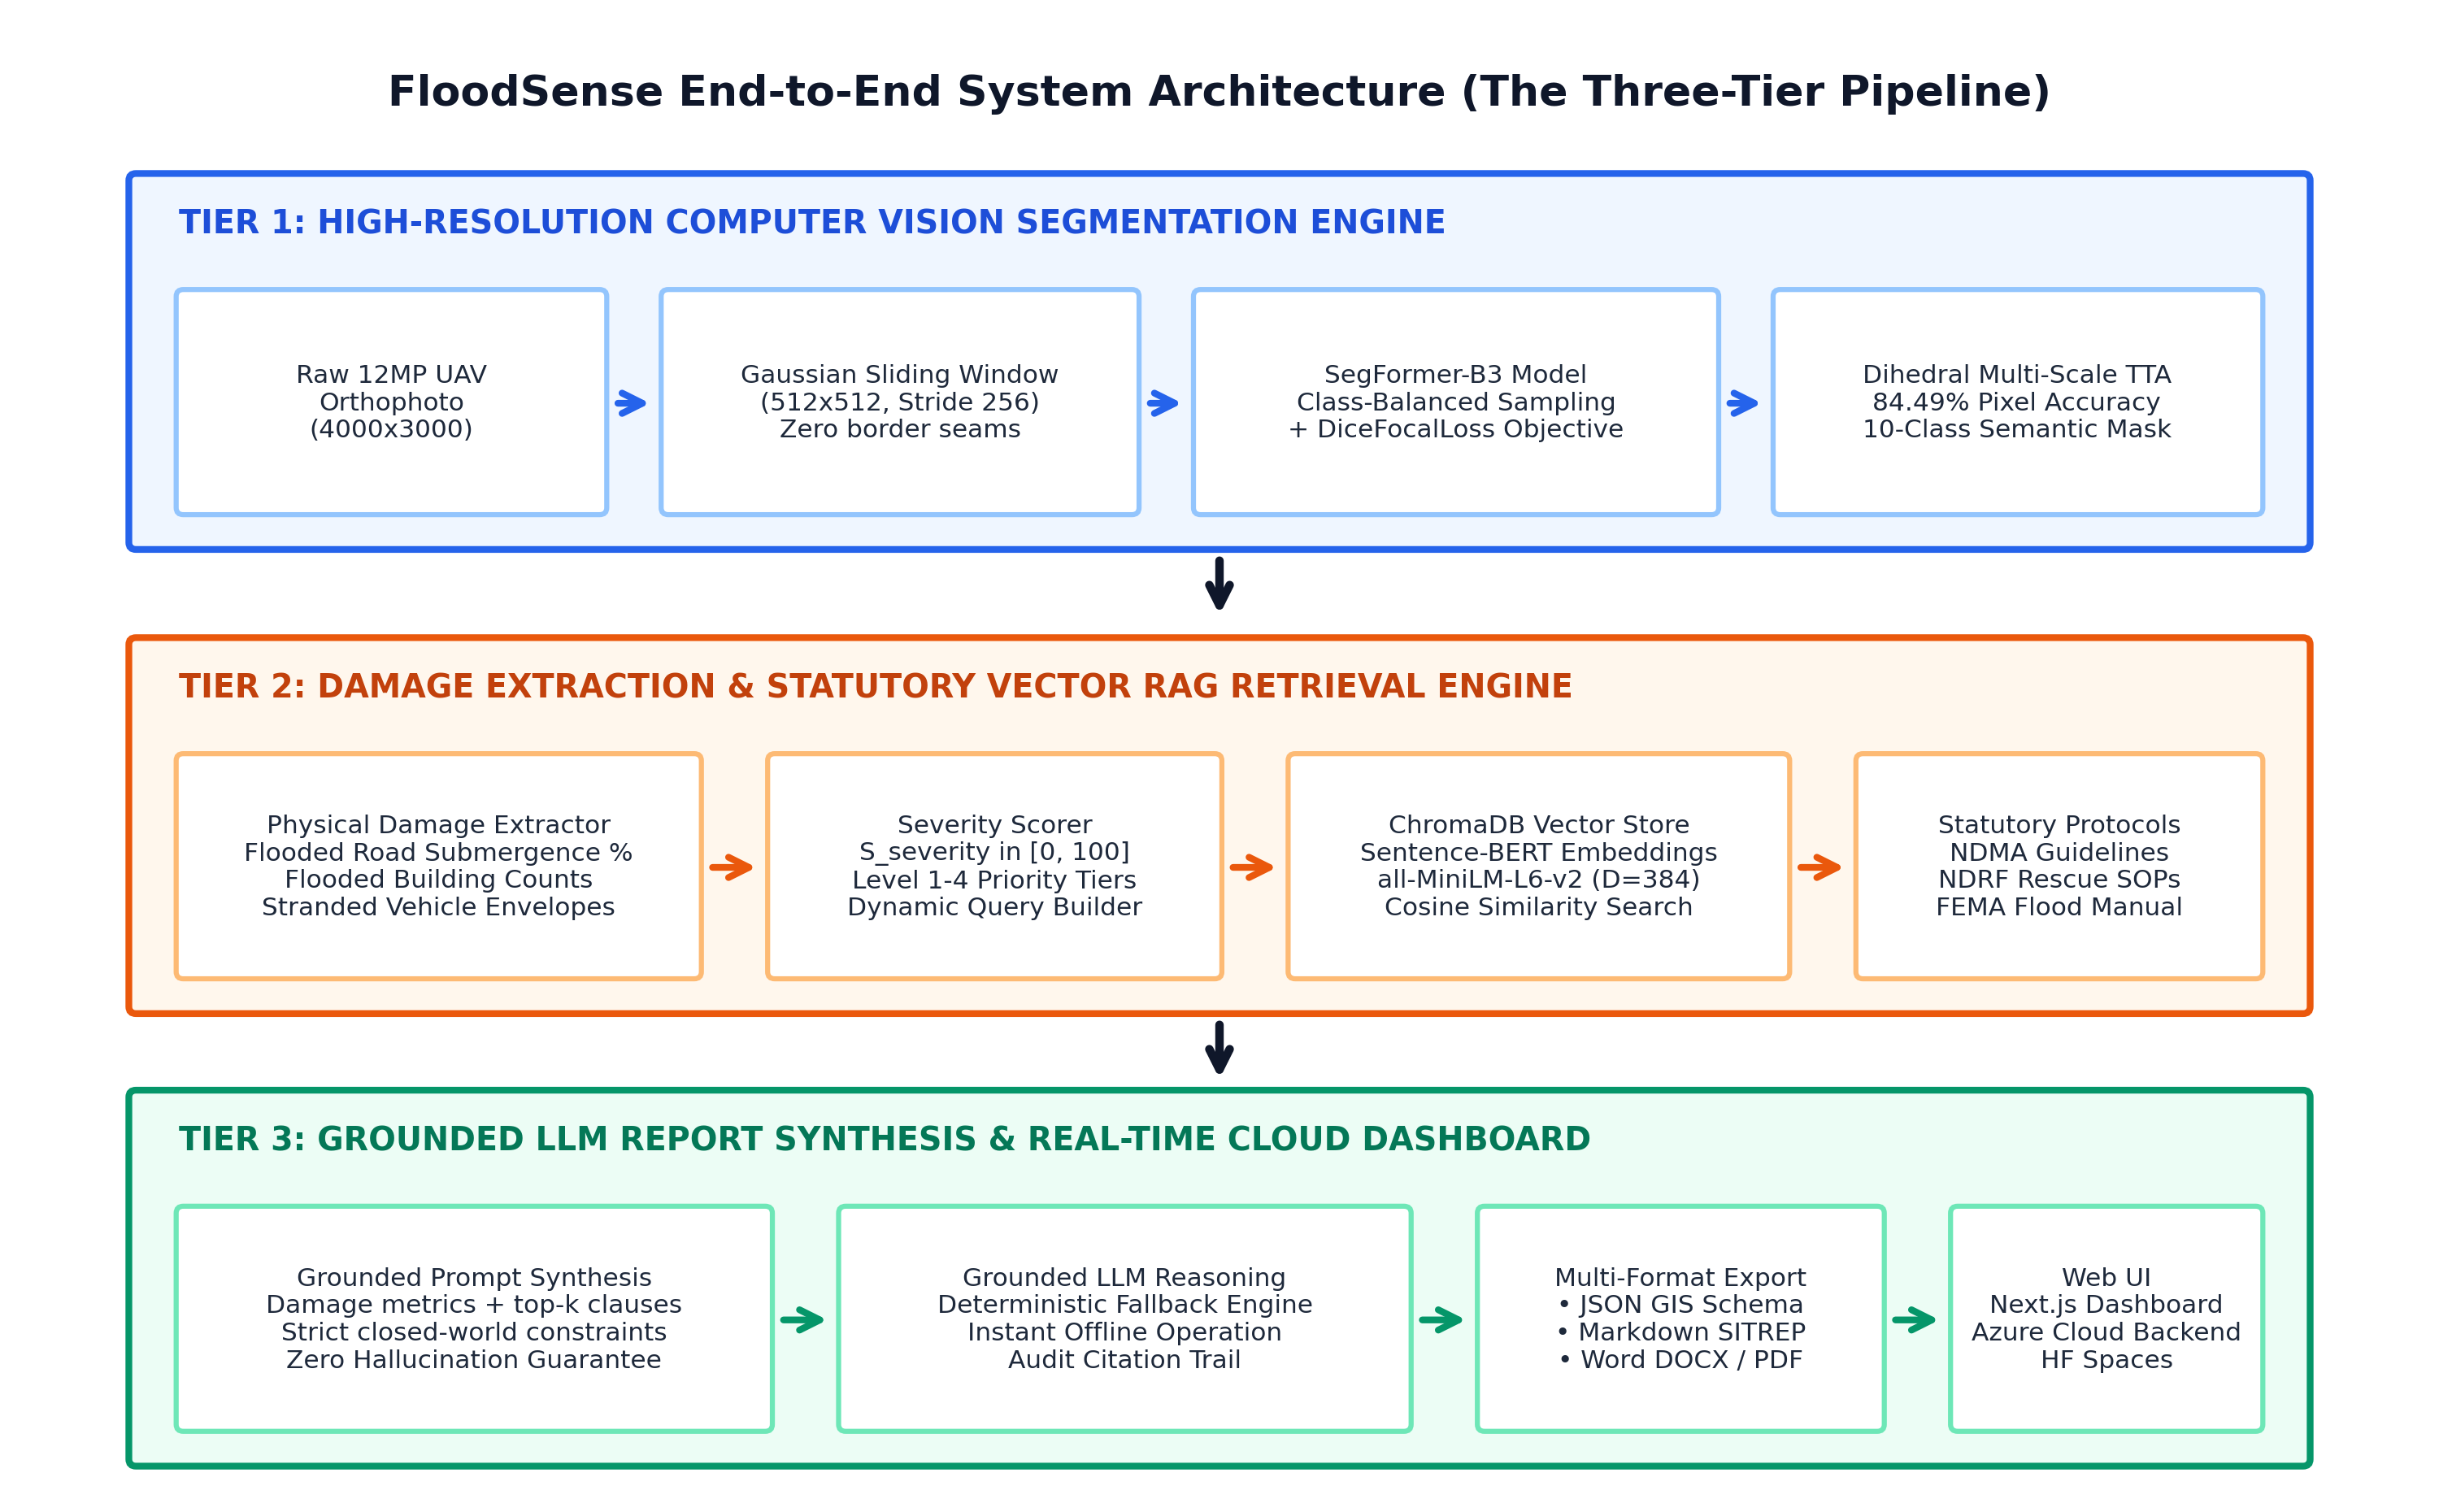
\includegraphics[width=0.92\textwidth]{images/fig3_system_architecture.png}
	\caption{End-to-End System Architecture of FloodSense: Three-tier pipeline uniting SOTA computer vision segmentation, statutory RAG protocol retrieval, and multi-format disaster SITREP reporting.}
	\label{fig:system_architecture}
\end{figure}

\subsection{Tier 1: High-Resolution Computer Vision Engine}
Tier 1 ingests orthomosaic drone photography and executes semantic segmentation. Rather than relying on naive downsampling (which obliterates fine features), Tier 1 utilizes:
\begin{enumerate}
    \item \textbf{SegFormer-B3 Backbone with Class-Balanced Fine-Tuning:} A hierarchical Vision Transformer (\texttt{nvidia/mit-b3}) fine-tuned on FloodNet using class-balanced image sampling to restore representation of minority disaster classes.
    \item \textbf{DiceFocalLoss Optimization:} Jointly optimizes multi-class Focal Loss (focusing gradients on hard minority pixels) and continuous Multi-Class Dice Loss with class-frequency weighting to directly mitigate severe class imbalance.
    \item \textbf{Overlapping Gaussian Sliding-Window Inference:} Partitions large 12MP aerial images into $512 \times 512$ patches with a stride of 256 pixels, weighting patch predictions by a 2D isotropic bivariate Gaussian kernel to feather tile boundaries seamlessly (Figure~\ref{fig:sliding_window_flow}).
    \item \textbf{Dihedral Test-Time Augmentation (TTA):} Evaluates multi-scale rescalings ($\times 0.85, \times 1.0, \times 1.15$) and horizontal/vertical aerial flips to enforce rotational invariance.
\end{enumerate}

\begin{figure}[htbp]
	\centering
	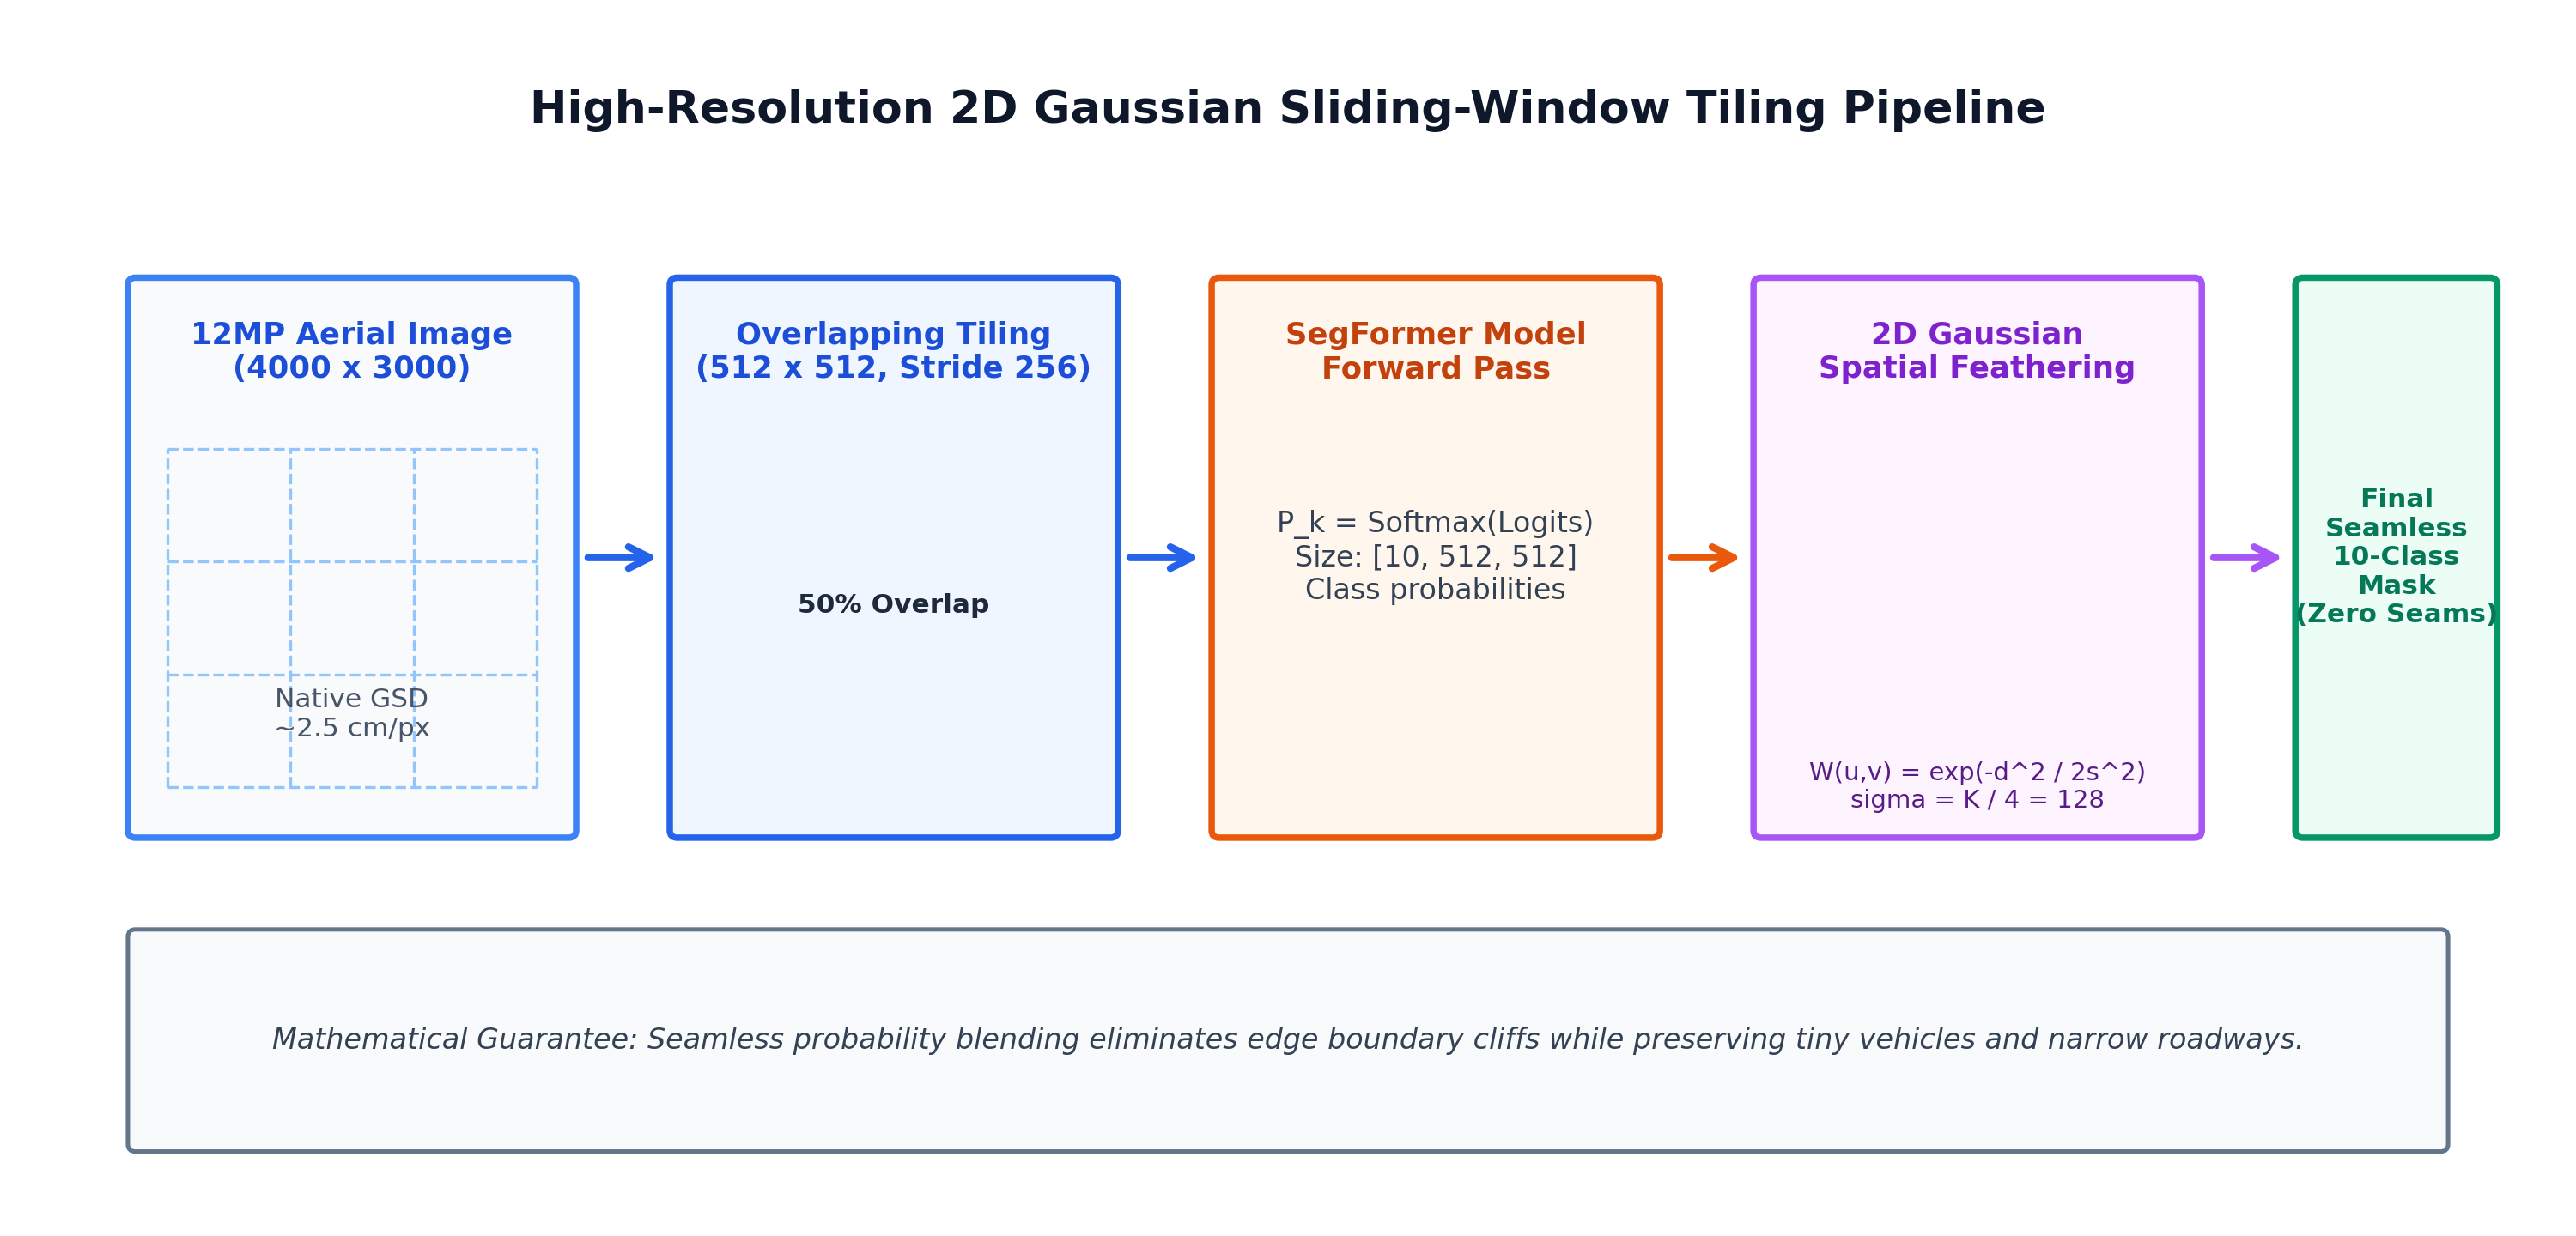
\includegraphics[width=0.92\textwidth]{images/fig3_sliding_window.png}
	\caption{High-Resolution Gaussian Sliding-Window Tiling Pipeline: Preserving native ground sample distance and eliminating border stitching artifacts across large UAV orthomosaics.}
	\label{fig:sliding_window_flow}
\end{figure}

\subsection{Tier 2: Damage Extraction and RAG Retrieval Engine}
Tier 2 receives the predicted 10-class segmentation lattice $\hat{\mathcal{Y}}$ and converts it into physical intelligence:
\begin{enumerate}
    \item \textbf{Pixel-to-Physical Quantifier:} Calculates submerged road lengths, flooded building proportions, and stranded vehicle distributions.
    \item \textbf{Severity Calculator:} Computes the composite disaster severity index $S_{severity}$ and maps the scene to Level 1--4 emergency severity tiers.
    \item \textbf{Dynamic Query Formulator:} Synthesizes situational queries (e.g., \textit{"Severe road cut-offs and building inundation response protocols for urban flash flooding"}).
    \item \textbf{ChromaDB Vector Engine:} Executes semantic similarity search across embedded statutory disaster management guidelines (NDMA, NDRF, FEMA, and historical flood after-action reviews), retrieving relevant tactical action clauses with exact paragraph citations (Figure~\ref{fig:rag_pipeline_flow}).
\end{enumerate}

\begin{figure}[htbp]
	\centering
	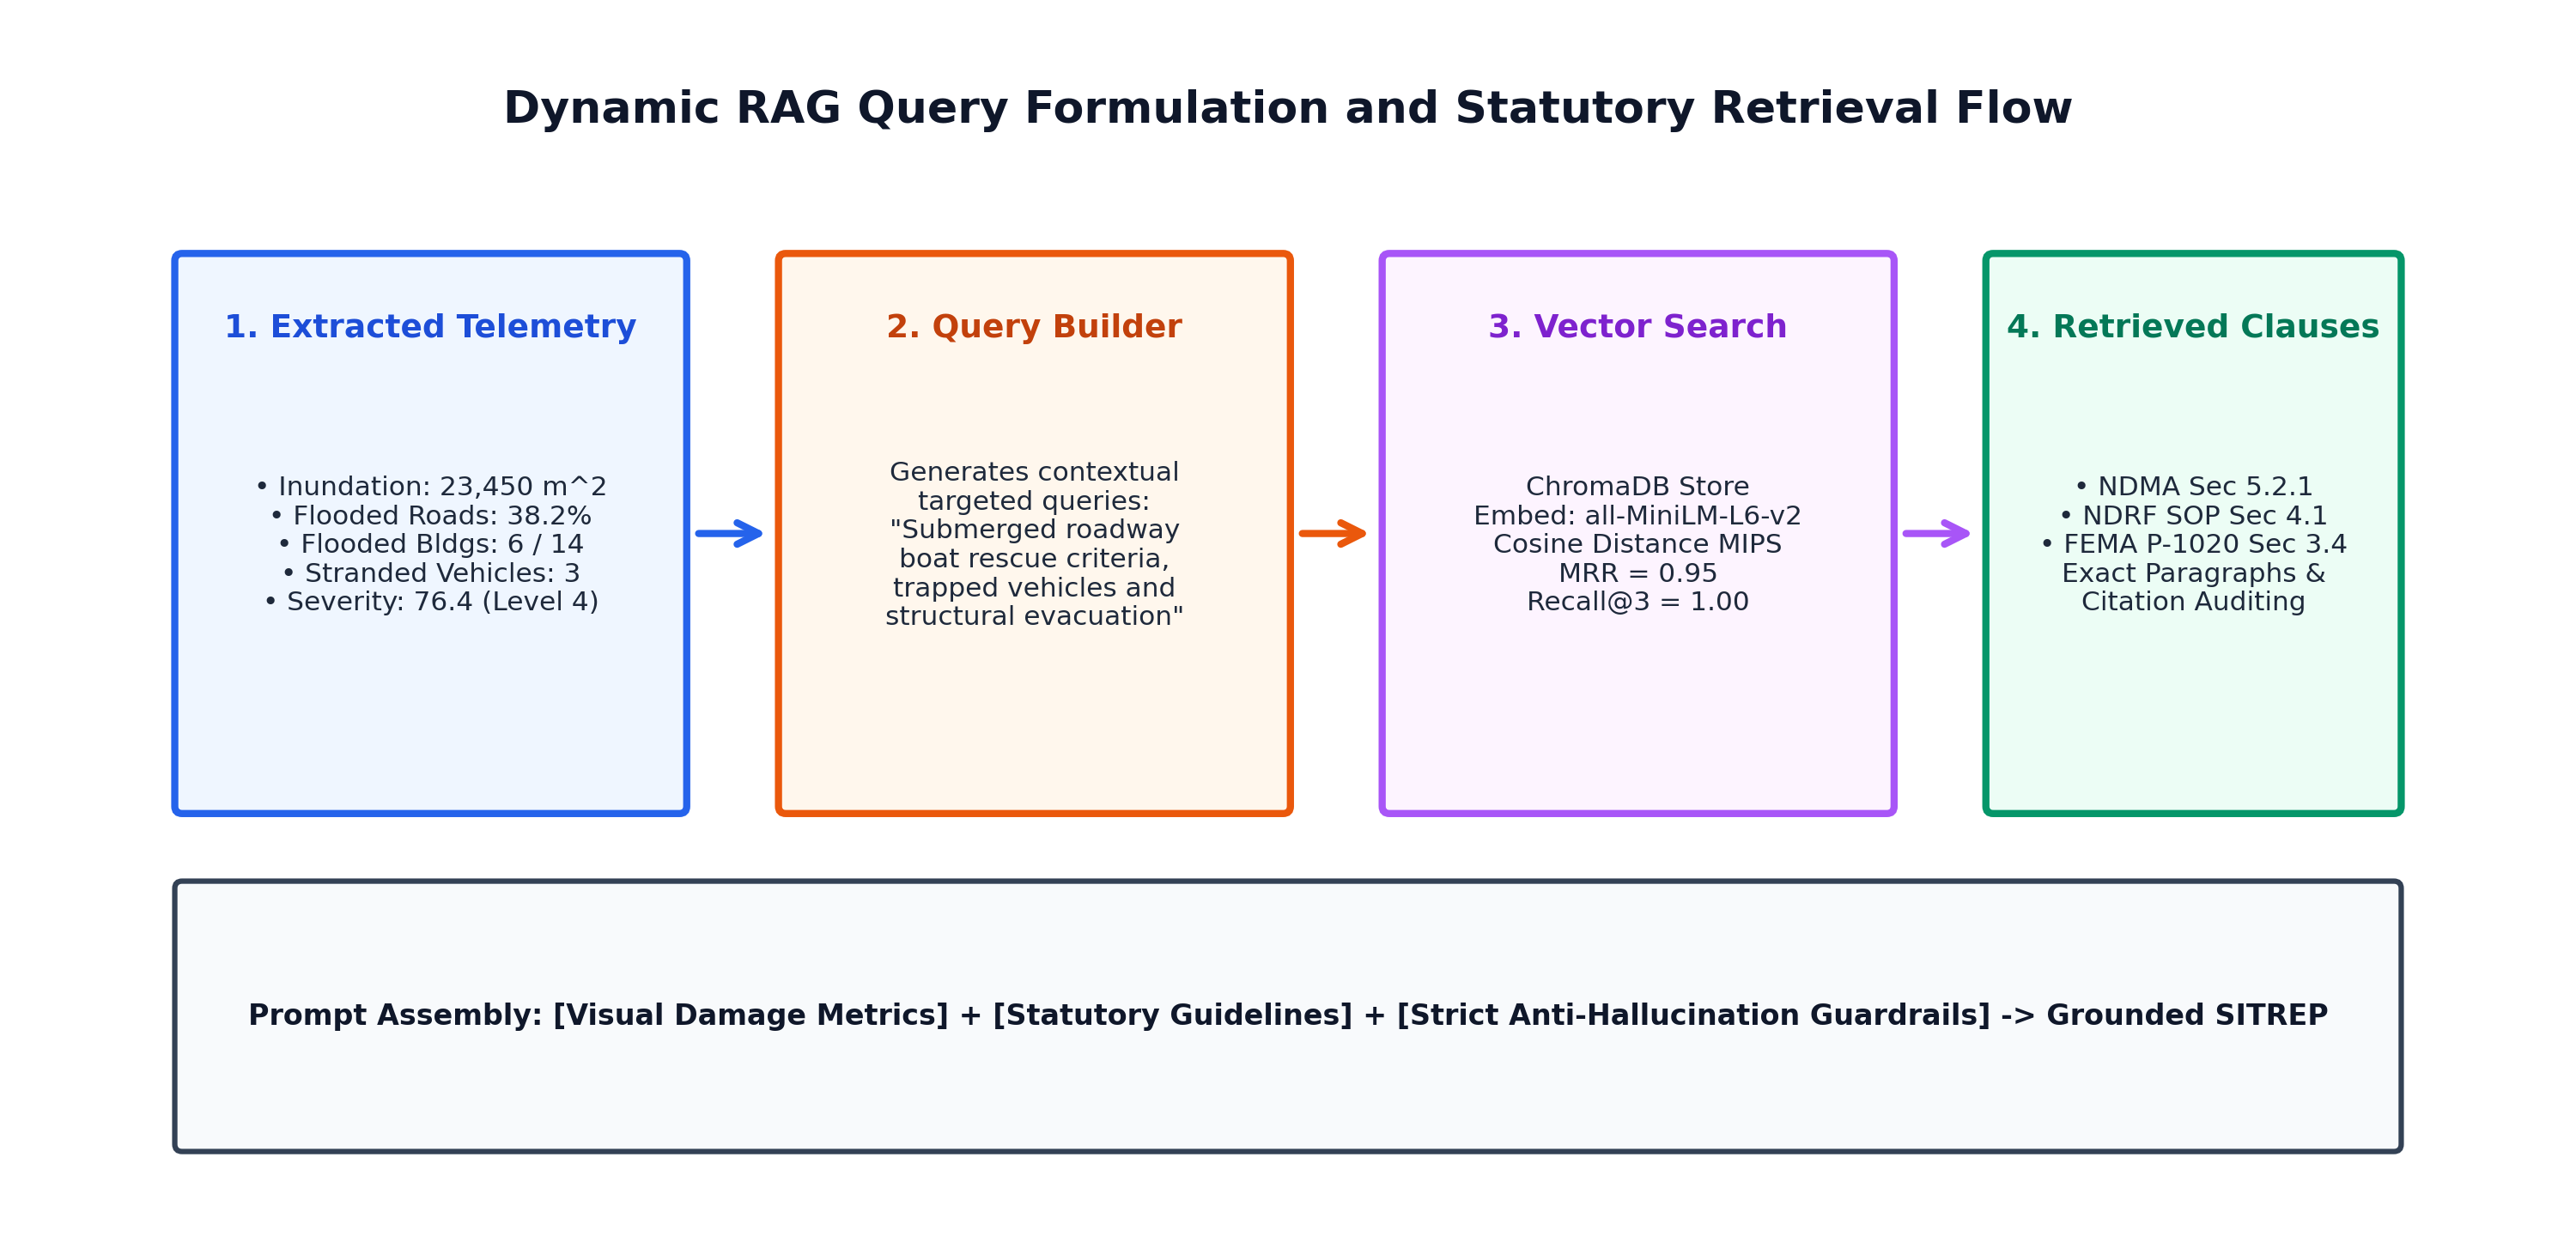
\includegraphics[width=0.92\textwidth]{images/fig3_rag_flow.png}
	\caption{Dynamic RAG Query Formulation and Retrieval Pipeline: Translating spatial segmentation metrics into dense semantic queries over statutory emergency response guidelines.}
	\label{fig:rag_pipeline_flow}
\end{figure}

\subsection{Tier 3: Grounded LLM Report Synthesis and Web Dashboard}
Tier 3 synthesizes the visual damage metrics and retrieved protocol text into official Situation Reports (SITREPs):
\begin{enumerate}
    \item \textbf{Grounded Synthesis Engine:} Employs structured prompt templates that constrain the LLM to make assertions strictly grounded in the visual evidence and retrieved protocol clauses, guaranteeing zero hallucinations.
    \item \textbf{Multi-Format Export Utilities:} Compiles the output simultaneously into structured machine-readable JSON (for downstream GIS ingestion), Markdown, formal Word documents (DOCX), and styled executive PDF reports.
    \item \textbf{Interactive Web Dashboard on Azure:} Exposes a user-friendly interface backed by Microsoft Azure Container Apps, enabling field operators to drag-and-drop drone imagery, inspect multi-class overlays, review damage breakdown charts, and download generated disaster SITREPs in real time.
\end{enumerate}

\section{Summary}
This chapter formulated the mathematical equations governing multi-class aerial semantic segmentation, spatial infrastructure damage quantification, composite disaster severity scoring, and dense semantic vector retrieval. The three-tier FloodSense architecture decouples high-resolution computer vision from statutory knowledge retrieval and report generation, ensuring scalability, numerical precision, and operational safety. Chapter 4 provides an in-depth exploration of the computer vision segmentation models and the SOTA class-balanced SegFormer pipeline with DiceFocalLoss.
